\chapter{Theoretical Background}
\label{chap:background}
\section{The Standard Model of Particle Physics}
\label{sec:standard_model}

\begin{figure}[ht]
  \centering
  \includegraphics[width=0.8\textwidth]{figures/standard_model.pdf}
  \caption{The particles of the Standard Model. Particle properties taken from reference~\cite{PDG2024}.}
  \label{fig:standard_model_particles}
\end{figure}

The Standard Model (SM) of particle physics is a quantum field theory describing three of the four fundamental interactions of nature—electromagnetic, weak and strong—and the elementary particles on which they act.

It is formulated as a renormalisable, Lorentz-invariant gauge theory with gauge group
\begin{equation}
  SU(3)_C \times SU(2)_L \times U(1)_Y  
\end{equation}
and its structure has been established in a series of seminal works~\cite{standardmodel0,standardmodel1,standardmodel2,standardmodel7,standardmodel5,standardmodel9}.
A summary of the particle content is shown in \cref{fig:standard_model_particles}.
The elementary particles fall into two categories, fermions and bosons. Fermions are spin-$\tfrac{1}{2}$ particles that constitute matter, organised into three generations of quarks and leptons.
Quarks carry colour charge and participate in the strong interaction; leptons do not.
Bosons are integer-spin gauge particles mediating the fundamental forces: the photon for electromagnetism, the $W^\pm$ and $Z$ bosons for the weak interaction, and eight gluons for the strong interaction.
The Higgs boson completes the SM and is responsible for electroweak symmetry breaking (EWSB), giving mass to the weak gauge bosons and, through Yukawa couplings, to the fermions.
The SM Lagrangian can be written schematically as 
\begin{equation}
    \mathcal{L}_\mathrm{SM} = \mathcal{L}_\mathrm{gauge}
  + \mathcal{L}_\mathrm{fermion}
  + \mathcal{L}_\mathrm{Yukawa}
  + \mathcal{L}_\mathrm{Higgs},
\end{equation}
where the first term contains the gauge kinetic terms and self-interactions, the second describes the fermions and gauge covariant derivatives, the third encodes the Yukawa couplings to the Higgs field, and the last term contains the Higgs potential and EWSB mechanism.
Below, the three interaction sectors are briefly summarised, with an emphasis on aspects relevant to top-quark physics and LHC phenomenology.

\subsection{Electromagnetic Interaction}
The electromagnetic interaction is described by quantum electrodynamics (QED), the $U(1)_{\mathrm{EM}}$ gauge theory that remains after EWSB. Its massless gauge boson, the photon, couples to electric charge and does not self-interact. Because QED is an Abelian theory, its coupling runs only mildly with energy and remains perturbative at all experimentally accessible scales.
\subsection{Weak Interaction}
The weak interaction, together with electromagnetism, forms the electroweak theory based on the gauge group $SU(2)_L \times U(1)_Y$. The vacuum expectation value of the Higgs field spontaneously breaks the symmetry to $U(1)_{\mathrm{EM}}$, giving masses to the weak gauge bosons through the Higgs mechanism~\cite{higgs1,higgs2,higgs3}. The resulting massive $W^\pm$ and $Z$ bosons mediate a short-range force. 

A defining property of the weak interaction is its \emph{chiral} structure: charged-current interactions couple only to left-handed fermions and right-handed antifermions. This feature, predicted in~\cite{Parity_Violation_Theory} and confirmed in the Wu experiment~\cite{WU_Exp}, leads to maximal parity violation and characteristic angular distributions of weak decay products. The vertex factor of the charged-current interaction is given by 
\begin{equation}
  \frac{-ig}{2\sqrt{2}} \gamma^\mu (1 - \gamma^5),
\end{equation}
where $g$ is the weak coupling constant and $\gamma^\mu$ are the Dirac matrices. The projection operator $(1 - \gamma^5)$ leads to a coupling exclusively to the left-handed components. Based on this, the left-handed particles are arranged in $SU(2)_L$ doublets, while the right-handed particles are singlets.

For quarks, the weak eigenstates $d',s',b'$ are not identical to their mass eigenstates $d,s,b$. Their mixing is described by the Cabibbo-Kobayashi-Maskawa (CKM) matrix~\cite{cabibbo,kobayashi_maskawa}, which enables flavour-changing coupling in charged-current interactions.

\subsection{Strong Interaction}
\label{sec:strong_interaction}
The strong interaction is described by quantum chromodynamics (QCD), a non-Abelian gauge theory with gauge group $SU(3)_C$. Quarks carry colour charge, while gluons carry colour and anticolour index, giving rise to self-interactions through three- and four-gluon vertices.
These features lead to two fundamental properties.

\paragraph{Asymptotic freedom}
The QCD coupling decreases at high momentum transfer~\cite{standardmodel6,standardmodel7}, allowing perturbative calculations of hard processes such as top-quark pair production. In the high-energy regime of the LHC, quarks and gluons effectively behave as quasi-free particles.

\paragraph{Confinement}
At low energies, the QCD coupling becomes large, preventing coloured states from existing in isolation. Instead, they form colour-neutral bound states--hadrons. The transition from short-distance partons to long-distance hadrons involves non-perturbative dynamics encapsulated through hadronisation models. These models cannot be obtained analytically and are a major source of uncertainty.

A crucial consequence for collider physics is that quarks and gluons produced in hard interactions undergo a cascade of QCD emissions before hadronising into jets. This process is typically
described in terms of:
\begin{itemize}
  \item \textbf{Parton distribution functions (PDFs)}, characterising the proton structure and
        entering via the QCD factorisation theorem~\cite{collins_soper_sterman}.
  \item \textbf{Initial- and final-state radiation (ISR/FSR)}, arising from soft and collinear
        gluon emission.
  \item \textbf{Parton showers}, which resum logarithmically enhanced emissions and are implemented
        in Monte Carlo generators such as \pythia, first developed
        in~\cite{SJOSTRAND1985321,parton_shower} and extended in modern
        formulations~\cite{pythia}.
  \item \textbf{Hadronisation models}, such as the Lund string
        model~\cite{lund_model,SJOSTRAND1984469}, which describe the confinement-driven formation
        of hadrons.
\end{itemize}


\subsection{Monte Carlo Simulation at Colliders}
\label{sec:mc_colliders}

\begin{figure}
  \centering
  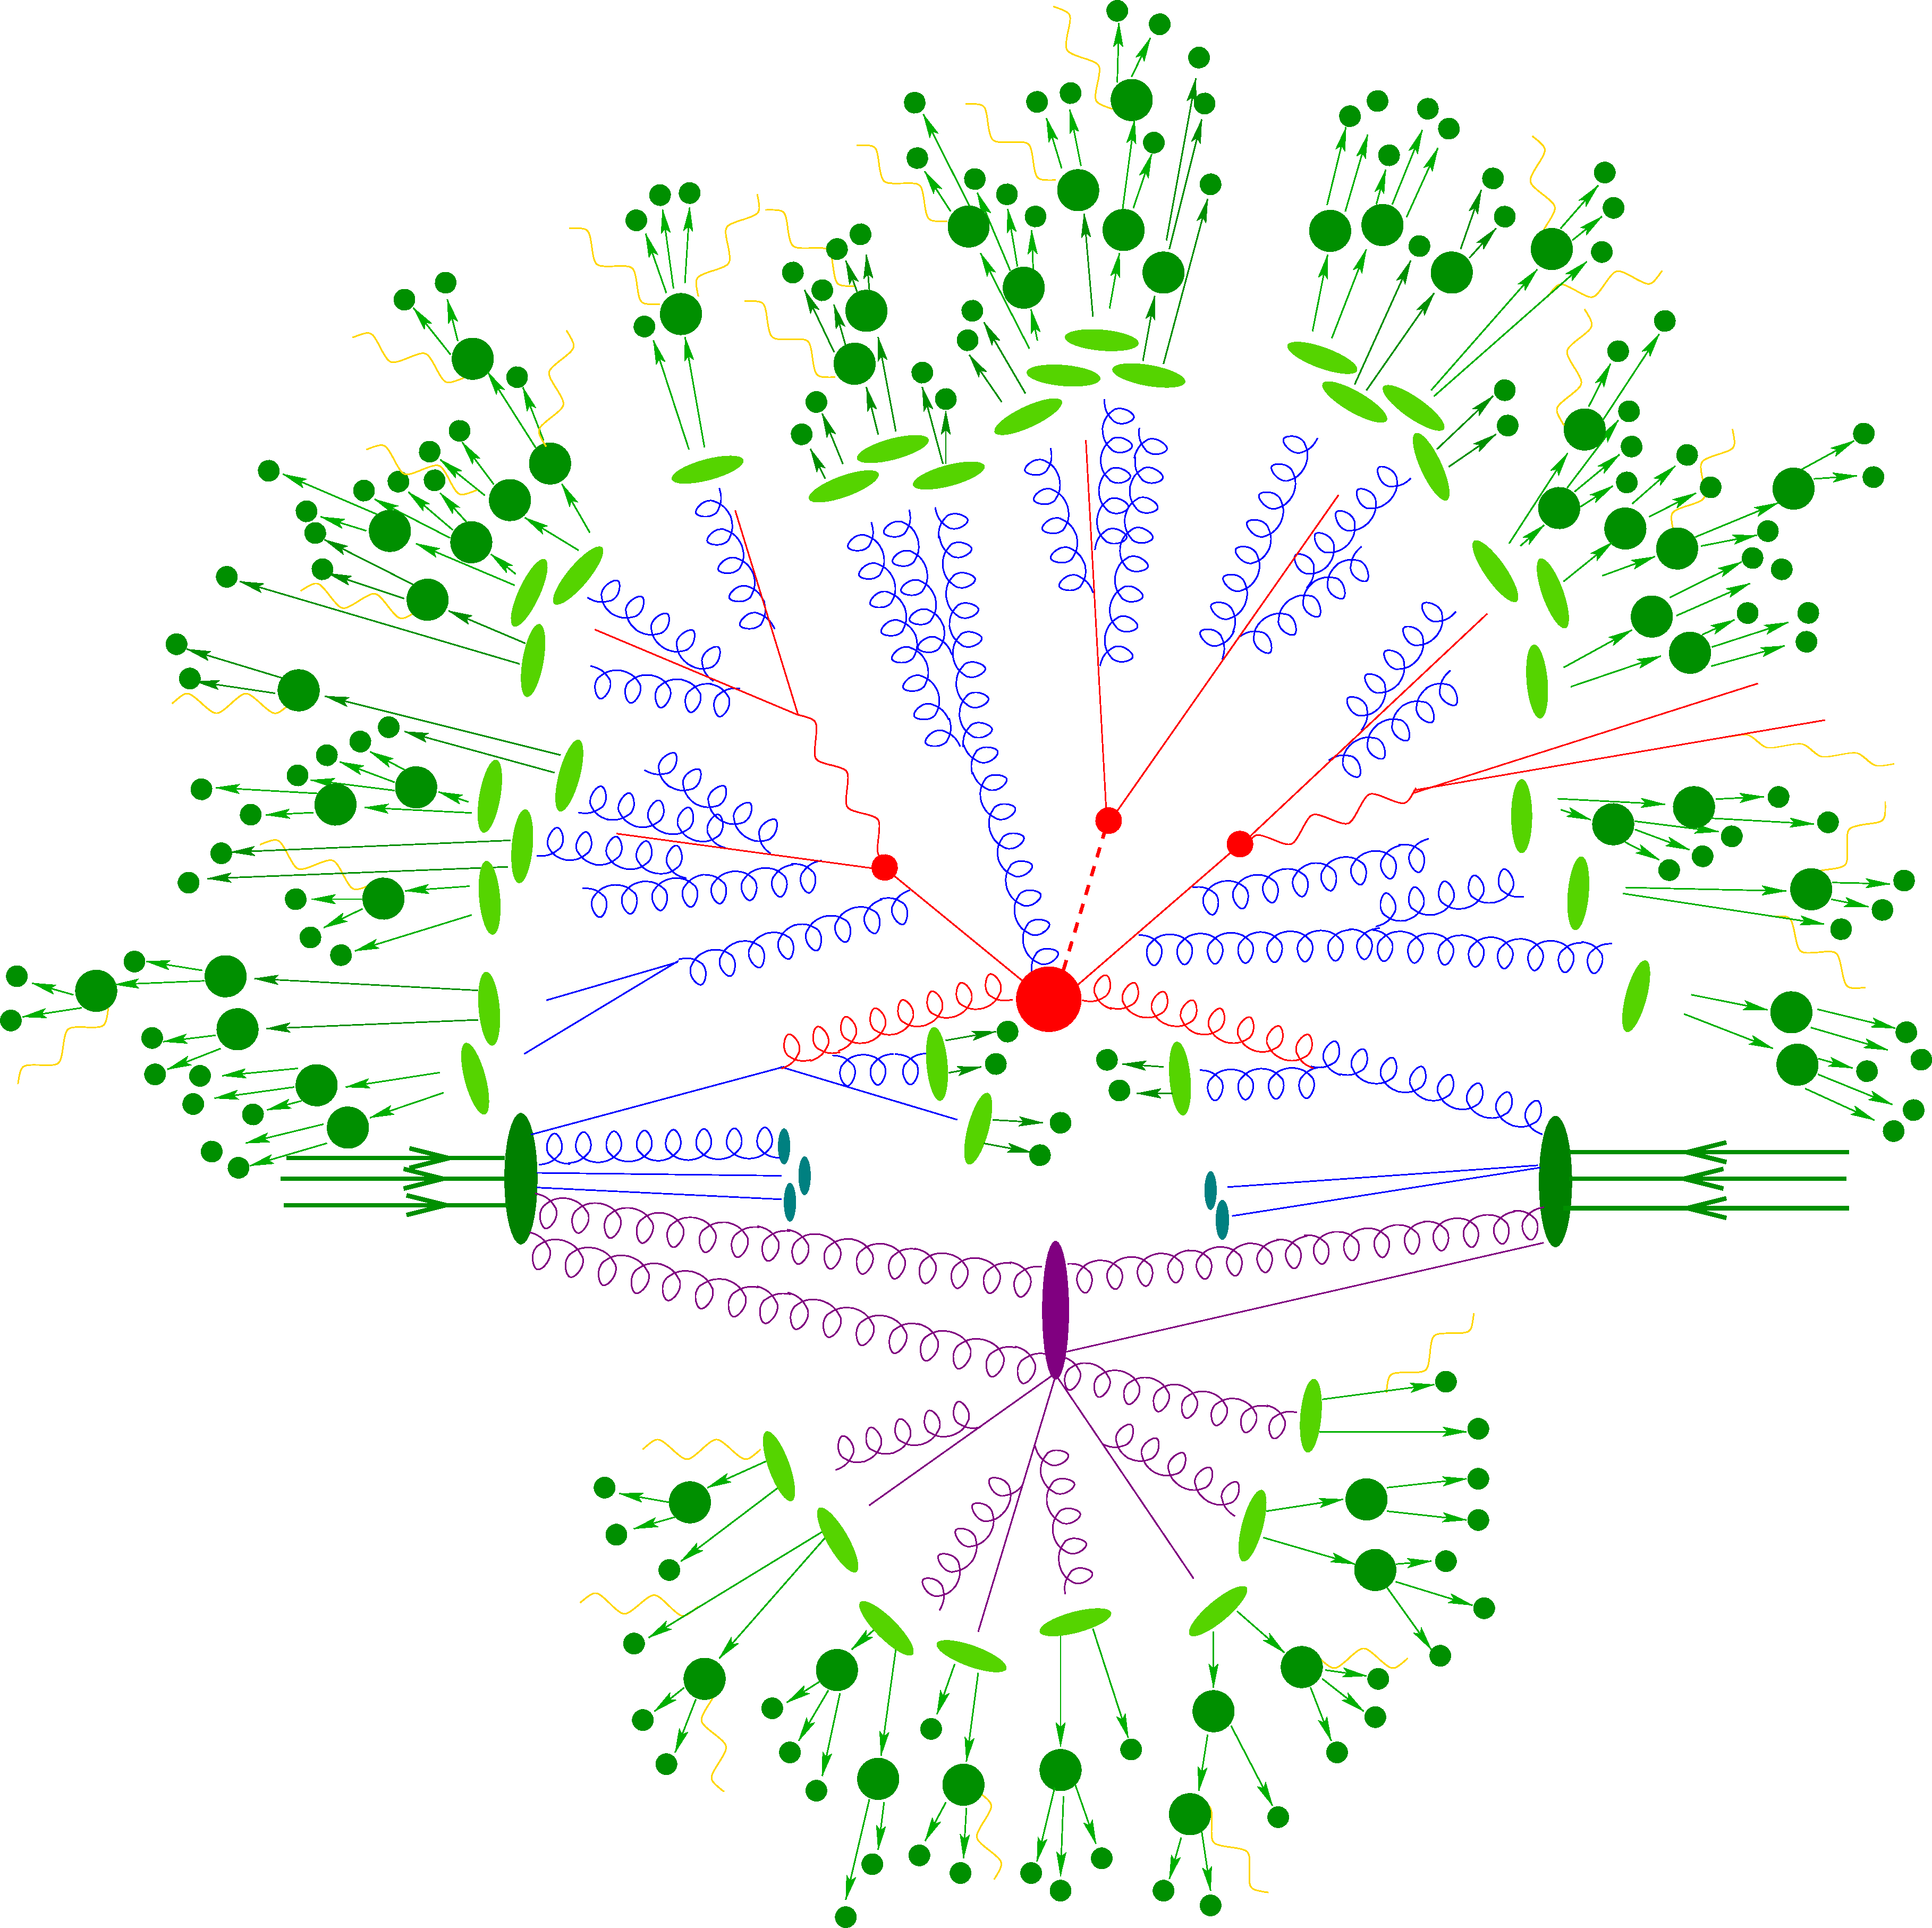
\includegraphics[width=0.6\textwidth]{figures/event_svg-tex.pdf}
  \caption{Schematic representation of the Monte Carlo event generation process in particle
           physics. Colouring of vertices and particles indicates the event generation stage:
           hard scattering process (big red blob), QCD radiation (blue), hadronisation (light
           green), showering (dark green), and a secondary vertex (purple).
           Taken from reference~\cite{sherpa_1}.}
  \label{fig:mc_stages}
\end{figure}
Building on the QCD processes introduced in \cref{sec:strong_interaction}, predictions at the \lhc are obtained almost exclusively via Monte Carlo (MC) simulations, in which event samples are generated by randomly sampling from the underlying probability distributions. The complex mathematical structure of the Standard Model, combined with the wide range of energy scales involved in collider processes, renders purely analytical predictions rarely feasible.

\paragraph{Hard scattering}
Events are simulated using a cascade of programs, each responsible for a distinct stage of the event. Matrix-element generators compute the hard-scattering amplitude for a given process and sample the kinematic phase space according to the differential cross-section, yielding the partonic final state of the hard interaction; events at this stage are referred to as
\textit{parton-level}.

\paragraph{Parton shower and hadronisation}
The parton-level events are subsequently passed through parton-shower and hadronisation algorithms, as outlined in \cref{sec:strong_interaction}, which evolve the hard-scatter partons into colour-neutral hadronic final states. A schematic description of the full event generation chain
is given in \cref{fig:mc_stages}.

\paragraph{Detector simulation}
Finally, detector simulation programs model the interactions of stable particles with the detector material, producing realistic detector responses. This includes simulating energy deposits in calorimeters, hits in tracking detectors, and other relevant signals. For many applications, a simplified fast simulation is sufficient, involving smearing of particle momenta and energies to match the detector resolution, applying efficiency corrections, and accounting for pile-up---the contribution from additional inelastic $pp$ interactions occurring within the same bunch crossing.


\section{Top-Quark Physics}
\label{sec:top-quark}
\begin{figure}[ht]
  \centering

  \begin{subfigure}[c]{0.3\textwidth}
    \centering
    \includegraphics[width=\textwidth]{figures/feynman-diagrams/ttbar_production_gg_t_channel.pdf}
    \caption{}
    \label{fig:top_production_gg_t_channel}
  \end{subfigure}
  \hfill
  \begin{subfigure}[c]{0.3\textwidth}
    \centering
    \includegraphics[width=\textwidth]{figures/feynman-diagrams/ttbar_production_gg_s_channel.pdf}
    \caption{}
    \label{fig:top_production_gg_s_channel}
  \end{subfigure}
  \hfill
  \begin{subfigure}[c]{0.3\textwidth}
    \centering
    \includegraphics[width=\textwidth]{figures/feynman-diagrams/ttbar_production_gg_u_channel.pdf}
    \caption{}
    \label{fig:top_production_gg_u_channel}
  \end{subfigure}
  \begin{subfigure}[b]{0.3\textwidth}
    \centering
    \includegraphics[width=\textwidth]{figures/feynman-diagrams/ttbar_production_qq_s_channel.pdf}
    \caption{}
    \label{fig:top_production_qq_s_channel}
  \end{subfigure}

  \caption{Leading order Feynman diagrams for top-quark pair production in \subrefb{fig:top_production_qq_s_channel}
     \subrefb{fig:top_production_gg_t_channel}, \subrefb{fig:top_production_gg_s_channel} \& \subrefb{fig:top_production_gg_u_channel} gluon fusion (ggF) and \subrefb{fig:top_production_qq_s_channel} quark-antiquark annihilation.}

  \label{fig:top_production}

\end{figure}

The top quark is the heaviest known elementary particle. The prediction of its existence arose due to the already established CP-Violation in the kaon system, which required a third generation of quarks to be explained within the SM framework~\cite{kobayashi_maskawa}. Furthermore, the discovery of the bottom quark in 1977~\cite{bottom_discovery} implied the existence of its weak isospin partner, the top quark. The top quark was eventually discovered in 1995 by the \cdf and \dzero collaborations at the \tevatron collider~\cite{top_discovery_cdf,top_discovery_d0}.
Currently, the world average of the top-quark mass is measured to be~\cite{PDG2024}
\begin{equation}
  m_t = 172.56 \pm 0.31~\unit{\giga\electronvolt}.
\end{equation}
Along with the largest mass, the top quark also has the strongest Yukawa coupling to the Higgs boson, making it interesting for studies of the Higgs mechanism and electroweak symmetry breaking.
Due to its large mass, the top quark also has the shortest lifetime of all quarks, about $5 \times 10^{-25}~\unit{\second}$~\cite{PDG2024}, which is shorter than the typical hadronisation timescale of $3 \times 10^{-24}~\unit{\second}$~\cite{hadronization_time_2}. Therefore, the top is the only quark that decays before it hadronises, allowing for direct studies of its properties through its decay products.

Notably, the top quark also decays before its spin can decorrelate, preserving spin information in the angular distributions of its decay products~\cite{spin_decorrelation_time}. This unique feature enables precise measurements of spin correlations and polarisation of top quarks.
At hadron colliders like the \lhc, top quarks are predominantly produced in pairs via the strong interaction.
The leading order (LO) Feynman diagrams for top-quark pair production are shown in \cref{fig:top_production}.
At the \lhc, the dominant production mechanism is gluon fusion (ggF).
This is due to the high gluon density in the proton at the relevant Bjorken-$x$ values for top-quark production and the low antiquark-contributions at a $pp$-collider.
The CKM matrix element $V_{tb}$ is close to unity~\cite{PDG2024}, leading to a nearly exclusive decay of the top quark into a $W$ boson and a $b$ quark.
The $W$ can subsequently decay either leptonically into a charged lepton and a neutrino or hadronically into a pair of quarks, with branching ratios of about $\text{BR}(W\to\ell,\nu)\approx1/3$ and $\text{BR}(W\to q\bar{q})\approx2/3$, respectively~\cite{PDG2024}.
Based on these $W$ decay modes, top-quark pair events are categorised into three channels. In the \textbf{dileptonic channel}, both $W$ bosons decay leptonically ($W^+ \to \ell^+ \nu_\ell$,$W^- \to \ell^-\bar{\nu}_\ell$), resulting in two charged leptons, two neutrinos and two $b$ quarks in the final state. This channel has a branching ratio of approximately $1/9$. The \textbf{semileptonic channel} occurs when one $W$ boson decays leptonically and the other hadronically ($W \to q\bar{q}'$), yielding one charged lepton, one neutrino, and four quarks (including two $b$ quarks) in the final state. Finally, in the \textbf{all-hadronic channel}, both $W$ bosons decay hadronically, producing six quarks (including two $b$ quarks) in the final state, which suffers from large multijet background contamination in the busy environment of hadron colliders like the \lhc. Both hadronic decays have a similar branching ratio of $4/9$.


\subsection{Spin Correlations in Top-Quark Pairs}
\label{sec:ttbar_entanglement}
As elaborated upon before, the top quark decays before it can hadronise or its spin decorrelates. Therefore, the spin information of the top quark is directly transferred to its decay products. In top-quark pair production, the spins of the top and antitop quarks are correlated due to the production mechanism. Due to the chiral nature of the weak interaction, these spin correlations manifest in the angular distributions of the decay products, particularly the charged leptons in the dileptonic decay channel.

Recent studies at the \lhc began to explore the potential effects of quantum entanglement in top-quark pairs~\cite{atlas_entanglement}. Entanglement generally describes a quantum mechanical phenomenon where the quantum states of two or more particles become correlated in such a way that the state of one particle cannot be described independently of the state of the other(s), even when the particles are separated by large distances~\cite{schrödinger_entanglement}. This property is expressed as the system having a non-separable density matrix. While a general description of this phenomenon is beyond the scope of this thesis, entanglement can be tested using specific criteria. One such criterion is the \emph{Peres-Horodecki criterion}~\cite{peres_criterion,entanglement_two_qbits}, which states that if the partial transpose of the density matrix of a bipartite system has at least one negative eigenvalue, then the system is entangled. Considering the top-quark pair's spin as a bipartite system of two spin-$\tfrac{1}{2}$ particles (qubits), this criterion can be applied to test for entanglement in their spin states.

In reference~\cite{entanglement_top_quarks}, it was proposed to measure entanglement in top-quark pairs produced at the \lhc by analysing the angular distributions of their decay products, specifically the charged leptons in the dileptonic decay channel. The study showed that by measuring the opening angle between the two leptons, one can construct an observable sensitive to the entanglement of the top quarks' spin system. Due to the kinematics of top-quark pair production, the entanglement is expected to be more pronounced in certain regions of phase space; one such region is at low invariant mass of the top-quark pair system.

One particular region of interest is the so-called \emph{threshold region}, referring to the region in which the invariant of ht \ttbar-system is close to the production threshold of $m(t\bar{t})\sim 350~\GeV$, where the top-quarks are produced with low relative velocity. In this region, the top-quark pair system is produced as a spin singlet state in about $\sim 80\%$ of the cases, leading to a strong entanglement signature~\cite{toponium_2}. The \atlas and \cms collaboration recently reported the first experimental evidence of quantum correlations consistent with entangled spin quantum states in top-quark pairs~\cite{atlas_entanglement,cms_entanglement}. Measurements of this variable are particularly sensitive in the dilepton channel, because the lepton has the highest spin-analysing power~\cite{spin_analyzing_power,spin_analyzing_power_jets}. The spin-analysing power measures the extent to which the spin information of the parent is imprinted in the angular distributions of the decay products. Due to QCD effects, this is lower for light jets compared to leptons.

\subsection{Top-Quark Pair Quasi-Bound-State Effects}
\label{sec:ttbar_toponium}
\begin{figure}[ht]
  \centering
  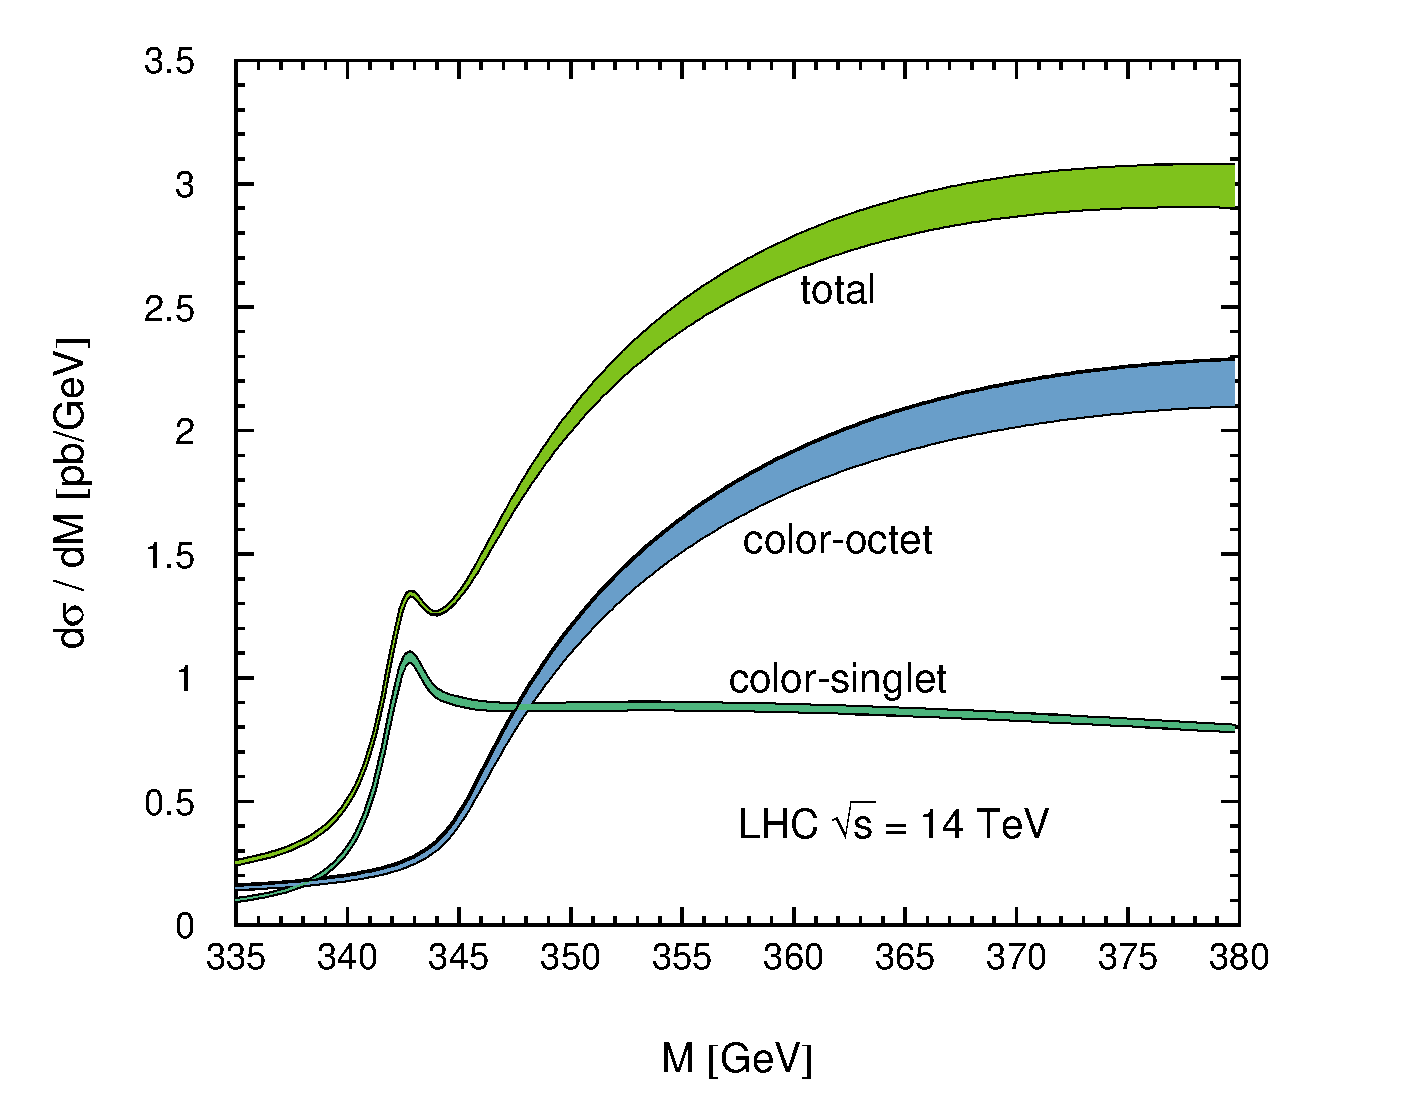
\includegraphics[width=.7\textwidth]{figures/toponium/xs2lhc14.pdf}
  \caption{Differential cross-section of top-quark pair production in     a colour-singlet or -octet state. The Figure is taken from     reference~\cite{toponium_2}, which provides further details on the   underlying modelling.}
  \label{fig:toponium_mttbar}
\end{figure}
Even though the top quark decays before it can hadronise, near the production threshold of top-quark pairs, the strong interaction between the top and antitop quarks can lead to the formation of transient bound states, coined as \textit{toponium}~\cite{toponium_1,toponium_2,toponium_3}. These bound state effects can influence the production cross-section and kinematic distributions of top-quark pairs near threshold. The \cms and \atlas collaborations have recently observed an excess in the invariant mass distribution of top-quark pairs near threshold, consistent with the presence of toponium-like bound state effects~\cite{CMS2025Pseudoscalar,atlas_toponium}. The modelling of these effects is based on non-relativistic QCD (NRQCD) calculations, which account for the strong interaction dynamics between the top and antitop quarks in the near-threshold region~\cite{NRQCD_toponium_1, NRQCD_toponium_2}. The leading contributions arise from the formation of colour-singlet $^1S_0$, which enhances the cross-section due to an attractive QCD potential. The differential cross-sections related to the different colour-states can be found in \cref{fig:toponium_mttbar}. A proper introduction to the physics behind this effect would exceed the scope of this thesis, which focuses on reconstruction techniques. Thus, for further reference, the reader is pointed to the aforementioned references \cite{NRQCD_toponium_1, NRQCD_toponium_2}.

Understanding and accurately modelling these bound-state effects is crucial for precision measurements of top-quark properties and for searches of new physics in top-quark pair production. One notable example is the measurement of quantum effects, where the strength of the observed entanglement properties is influenced by bound-state effects and by their impact on the spin structure of the top-quark pair system. The measurement of these effects relies on reconstructing the top-quark system at the production threshold and uses angular correlations among the top-quark's decay products, similar to studies of quantum effects.
\subsection{Dileptonic Decay Channel}
\label{sec:top_decay_modes}
\begin{figure}[ht]
  \centering
  \includegraphics[width=0.5\textwidth]{figures/feynman-diagrams/g_to_dilepton.pdf}
  \caption{Leading order Feynman diagram for top-quark pair   production via gluon fusion with dileptonic decay.}
  \label{fig:dilepton_ttbar_decay}
\end{figure}

While having the lowest branching ratio and thus the lowest event yields of all decay channels, the dilepton channel offers a particularly clean signature with reduced background contamination.
Furthermore, leptons can be reconstructed and identified with a high efficiency in a hadron-collider environment and carry charge information, which enables assignment to top or antitop quark, respectively.
This makes it very suited for precision measurements of top-quark properties. The presence of two neutrinos in the final state leads to missing transverse energy (\met) in the event, complicating the full reconstruction of the top quarks' kinematics. Advanced techniques, such as kinematic fitting and multivariate analyses, are often employed to address these challenges and extract maximum information from the dileptonic events.

\subsubsection{Kinematic Constraints}
\label{sec:kinematic_constraints}
Assuming both $W$ bosons and top quarks are on-shell, the following kinematic constraints can be applied to the dileptonic decay channel, 
\begin{alignat}{2}
  (\vec{p}_{\nu_1} + \vec{p}_{\nu_2})_{x} & = \met_x, &
  (\vec{p}_{\nu_1} + \vec{p}_{\nu_2})_{y} & = \met_y,  \label{eq:met}\\
  (p_{\ell_1} + p_{\nu_1})^2 & = m_W^2,  & (p_{\ell_2} + p_{\nu_2})^2 & = m_W^2, \label{eq:w_boson}    \\
  (p_{b_1} + p_{\ell_1} + p_{\nu_1})^2    & = m_t^2,\quad   & (p_{b_2} + p_{\ell_2} + p_{\nu_2})^2 & = m_t^2\,.\label{eq:top_quark_mass}
\end{alignat}
If one assumes the neutrinos to be massless, these six equations provide constraints on the six unknown components of the two neutrino momenta. Due to the algebraic nature of the constraints, multiple solutions can exist for a given event, leading to ambiguities in the reconstruction. Furthermore, the effects of detector resolution and off-shell particles can lead to the system of equations having no real-valued solution~\cite{sonnenschein_method, ellipse_method}. This motivates the development of more sophisticated reconstruction methods.

\subsection{Spin-Sensitive Angular Variables}
\label{sec:spin_sensitive_variables}
\begin{figure}[ht]
  \centering
  \begin{subfigure}[c]{0.49\textwidth}
    \centering
    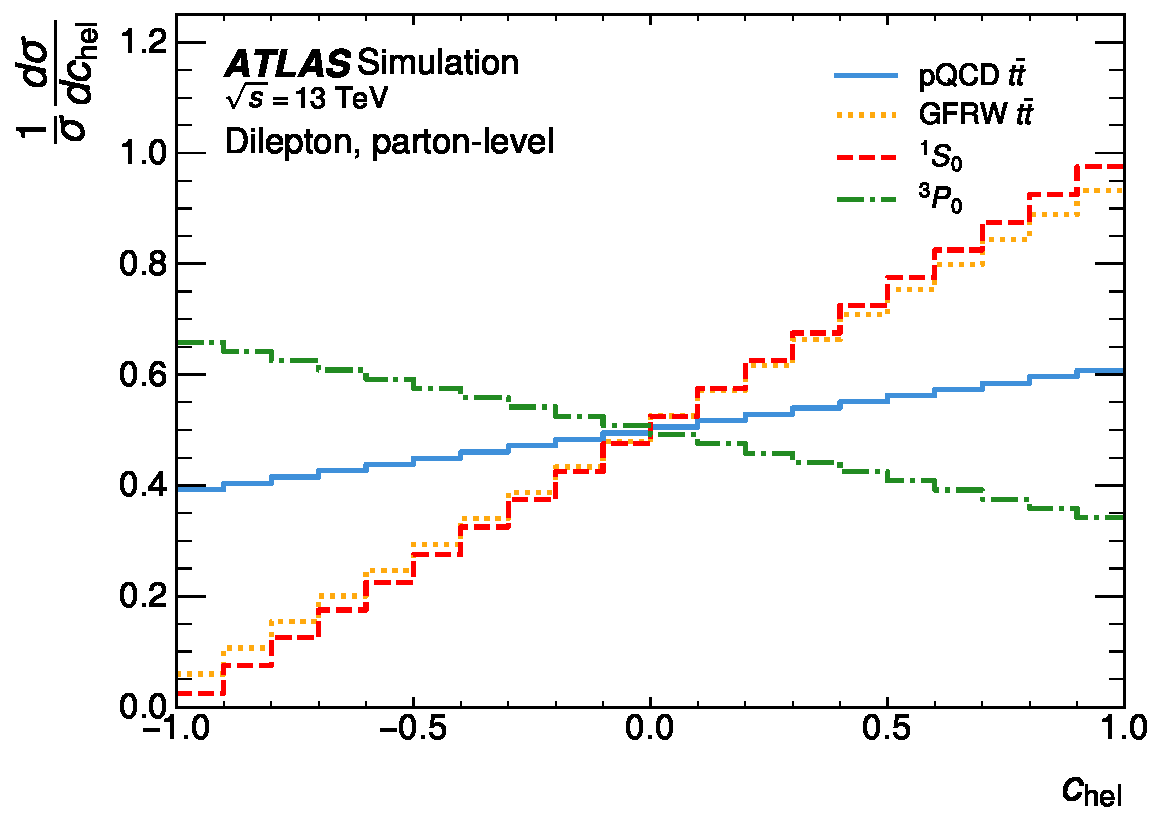
\includegraphics[width=\textwidth]{figures/c_hel_theory.pdf}
    \caption{\chel}
    \label{fig:c_hel_theory}
  \end{subfigure}
  \hfill
  \begin{subfigure}[c]{0.49\textwidth}
    \centering
    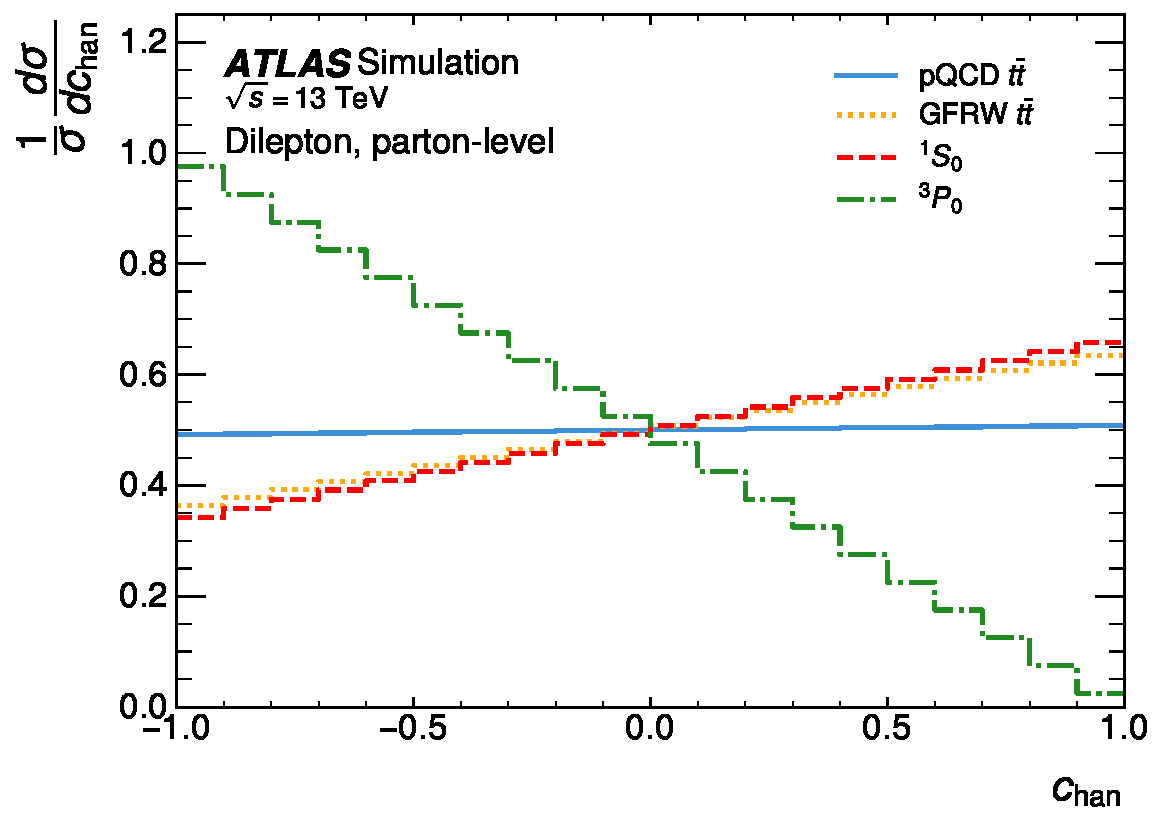
\includegraphics[width=\textwidth]{figures/c_han_theory.pdf}
    \caption{\chan}
    \label{fig:c_han_theory}
  \end{subfigure}
  \caption{Simulation of the distributions of  \chel and \chan for dileptonic decaying top-quark pairs produced near threshold. Distributions are shown for different spin states, as well as calculations using perturbative QCD (pQCD) or a modelling of the quasi-bound-state effects using a Green's Function Reweighting (GFRW)~\cite{NRQCD_toponium_2}. The distributions are normalised to unity and computed at parton level. The Figures are taken from   reference~\cite{atlas_toponium}.}
  \label{fig:spin_sensitive_theory}
\end{figure}


To study spin correlations and entanglement in top-quark pairs, a spin-sensitive angular variable is used. To measure quasi-bound-state effects, an additional angular variable is employed. Both variables are defined using the charged leptons from the dileptonic decay of the top-quark pair.

To compute the variables, top quarks and leptons are first boosted to the rest frame of the \ttbar system.

Their momentum vectors are boosted once more into their respective parent top quarks' rest frame. The normalised vectors of these transformed momenta are labelled as $\hat \ell_{t}^+$ and $\hat \ell^-_{t}$. The inner product of these unit vectors then defines the variable \begin{equation}
  \label{eq:c_hel}
  c_{\text{hel}} = \hat \ell_{t}^+ \cdot \hat \ell_{t}^-\,.
\end{equation}
Analogously, one can define the variable \chan, where either of the lepton momenta components parallel to the parent top-quark momentum in the \ttbar rest frame is flipped before taking the inner product \cite{bernreuther_nlospin_2004,bernreuther_spin_observables}. This variable adds important context by enabling isolation of scalar states. The differential cross-section of the spin-states as a function of \chel or \chan are obtained from simulation and found in \cref{fig:spin_sensitive_theory}. The distributions clearly show the distinctive shapes of the different spin states. Further, a stark difference between the slope of the perturbative QCD computation and the modelling of the quasi-bound state can be found, referred to as pQCD \ttbar and GFRW \ttbar in the plots, respectively.
This highlights the variables' sensitivity to the spin structure of the \ttbar system.

